%!TEX root = main.tex

\renewcommand{\u}{\cup}
\newcommand{\n}{\cap}
\newcommand{\stcut}{($s$,$t$)-cut}
\newcommand{\stcuts}{($s$,$t$)-cuts}
\newcommand{\refeq}[1]{(\ref{#1})}

\problem{2}

Let the be a flow network $G=(V,E)$ where $(S,T)$ and $(S',T')$ are minimum cuts.

For the beginning let's prove that $(S \n S', T \u T')$ and $(S \u S', T \n T')$ are \stcuts{}.
Since $(S,T)$ and $(S',T')$ are \stcuts{}, we know that the following properties are true:
\begin{equation}
S \u T = V \text{, } S \n T = \emptyset \text{ and }
S' \u T' = V \text{, } S' \n T' = \emptyset
\label{eq:start}
\end{equation}
First, let's prove that the same properties hold for $(S \n S', T \u T')$:
\begin{proof}
\begin{align}
(S \n S') \n (T \u T') &= [(S \n S') \n T] \u [(S \n S') \n T'] = \nonumber \\ 
&= \underbrace{(S \n T)}_{=\emptyset} \n (S' \n T) \u (S \n T') \n \underbrace{(S' \n T')}_{=\emptyset}) = \emptyset \label{eq:first-cut-empty-set}
\end{align}
and
\begin{align}
(S \n S') \u (T \u T') &= [(S \n S') \u T] \u [(S \n S') \u T'] = \nonumber \\
&= [\underbrace{(S \u T)}_{=V} \n (S' \u T)] \u [(S \u T') \n \underbrace{(S' \u T')}_{=V}] \label{eq:temp1}
\end{align}
From the definition we know that $S$, $S'$, $T$ and $T'$ are subsets of $V$, therefore we can write equation~\eqref{eq:temp1} as:
\begin{align}
(S \n S') \u (T \u T') &= (S' \u T) \u (S \u T') = \nonumber \\
&= S' \u S \u T \u T' = V. \label{eq:first-cut-vertex}
\end{align}
From \eqref{eq:first-cut-empty-set}~and~\eqref{eq:first-cut-vertex} we can say that $(S \n S', T \u T)$ is an \stcut{}.
\end{proof}

In an analogous fashion we can prove that $(S \u S', T \n T')$ is an \stcut{}:
\begin{proof}
\begin{align}
(S \u S') \n (T \n T') &= [(S \u S') \n T] \n [(S \u S') \n T'] = \nonumber \\ 
&= \underbrace{(S \n T)}_{=\emptyset} \u (S' \n T) \n \underbrace{(S \n T') \u \underbrace{(S' \n T')}_{=\emptyset}}_{=V} = \emptyset = \nonumber \\
&= (S' \n T) \u (S \n T') = (S \u S') \n (T \u T') = \emptyset \label{eq:second-cut-empty-set}
\end{align}
and
\begin{align}
(S \u S') \u (T \n T') &= [(S \u S') \u T] \n [(S \u S') \u T'] = \nonumber \\
&= \underbrace{(S \u T)}_{=V} \u (S' \u T) \n (S \u T') \u \underbrace{(S' \u T')}_{=V} = \nonumber \\
&= V \n V = V \label{eq:second-cut-vertex}
\end{align}

From \eqref{eq:second-cut-empty-set}~and~\eqref{eq:second-cut-vertex} we can conclude that $(S \u S'), (T \n T')$ is an \stcut{}.
\end{proof}

We now need to prove that $(S \n S', T \u T')$ and $(S \u S', T \n T')$ are minimum \stcuts{}.
Since $(S, T)$ and $(S', T')$ are minimum \stcuts{} the follow property holds:
\begin{equation}
| f^{*} | = \| S, T \| = \| S', T' \|
\label{eq:minimum-cuts}
\end{equation}
First, let's split our vertexes into 4 sets, as shown in figure~\ref{fig:problem2}. 

\begin{figure}[h!bt]
	\begin{center}
	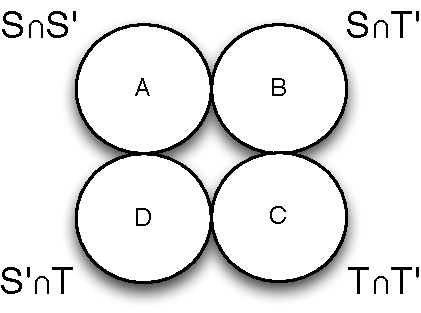
\includegraphics{problem2}
	\end{center}
	\caption{Splitting the vertex set into 4 disjoint sets}
	\label{fig:problem2}
\end{figure}

This gives us four subsets:
\begin{align}
A &= S \n S' \\
B &= S \n T' \\
C &= S' \n T \\
D &= T \n T' 
\end{align}

This allows us to rewrite equation~\ref{eq:minimum-cuts} as:
\begin{equation}
|f^{*}| = \| A \u B,  C \u D \| = \| A \u D, C \u B \|
\label{eq:breaking-the-flow}
\end{equation}
Since $(S \n S', T \u T')$ should be a minimum cut, this means that the following must hold true:
\begin{equation}
|f^{*}| = \| S \n S', T \u T' \| = \| A, B \u C \u D \|
\label{eq:breaking-the-flow-intersect}
\end{equation}
Let's prove this:
\begin{proof}
First, we can break the flow $\|S,T\|$ as:
\begin{equation}
\| S, T \| \overset{(\ref{eq:breaking-the-flow})}{=} \| A \u B , C \u D \| = \| A, B \u C \u D \|
\end{equation}
If we use equations (\ref{eq:breaking-the-flow}) and (\ref{eq:breaking-the-flow-intersect}) we come to the following equality:
\begin{equation}
\| A, B \u C \u D \| = \| A \u B, D \u C \|
\end{equation}
We can rewrite it as:
\begin{equation}
\| A, B \| + \| A, C \| + \| A, D \| = \| A, D \| + \| A, C\| + \| B, D \|  + \| B, C \|
\end{equation}
which we simplify to
\begin{equation}
\| A, B\| = \| B, D \| + \| B, C \|
\label{eq:simplified-flow}
\end{equation}

From the conservation law, we know that $\delta f(v)=0, \forall v \in V \setminus \{s,t\}$.
Since ${s,t} \notin B$ and ${s,t} \notin D$, from the conservation law we can deduce that 
\begin{equation}
\| B, D \| = 0
\label{eq:bd-is-zero}
\end{equation}

Since $s \in A$, from the conservation law we can deduce that $\delta A = |f^{*}|$. Also, since $\{s, t \} \notin B$ we can define the flow from $A$ to $B$ as:
\begin{equation}
\| A, B \| = |f^{*}|
\label{eq:ab-is-f}
\end{equation}

Similarly, since $t \in C$ and $t \notin B$, using the conservation law, we can define the flow from $B$ to $C$ as:
\begin{equation}
\| B, C \| = |f^{*}|
\label{eq:bc-is-f}
\end{equation}

From equations \refeq{eq:bd-is-zero}, \refeq{eq:ab-is-f} and \refeq{eq:bc-is-f}, we can write equation \refeq{eq:simplified-flow} as:
\begin{equation}
|f^{*}| = |f^{*}|,
\end{equation}
which is true. 

We can therefore conclude that $(S \n S', T \u T')$ is a minimum \stcut{} in G.
\end{proof}

Analogously, we can prove that $(S \u S', T \n T')$ is minimum \stcut{}.
\begin{proof}
Using the same subsets shown in figure~\ref{fig:problem2}, we can write the flow $\| S \u S', T \n T' \|$ as:
\begin{equation}
\| S \u S', T \u T' \| = \| A \u B \u D, C \|
\end{equation}
This can be rewritten as :
\begin{equation}
\| S \u S', T \n T' \| = \| A, C \| + \| B, C \| + \| D, C \|
\end{equation}
From the conservation law we know that $\| A, C \| = -|f^{*}|$ and $\|B, C\| = \|D, C\| = |f^{*}|$.
Therefore,
\begin{equation}
\| S \u S', T \n T' \| = |f^{*}|
\end{equation}
This shows that $(S \u S', T \n T')$ is a minimal \stcut{}.
\end{proof}
